% Chapter Template

\chapter{Data} % Main chapter title

\label{Chapter3} % Change X to a consecutive number; for referencing this chapter elsewhere, use \ref{ChapterX}

%----------------------------------------------------------------------------------------
%	SECTION 1
%----------------------------------------------------------------------------------------

\section{Dataset}

The dataset used to train and test the machine learning model was obtained from another paper that was working on a similar project. The authors of that paper made their dataset available online. There are 2252 songs in this dataset, 1802 of which had been categorised as the training set while the rest had been categorised as the test set. Each song is in major key and only have a single chord per bar. For each song, all the relevant features had been extracted and placed into a single \emph{CSV} file. These files can then be read and converted to DataFrame format using Python \emph{Pandas} as shown in Figure \ref{fig:CSV_DF}.

As can be seen in Figure \ref{fig:CSV_DF}, the rows each contain information about a single note. Each bar is taken to be a single measure. The columns each represent a different piece of information about that particular note. \emph{time} refers to the time signature, \emph{measure} refers to the measure to which that particular note belongs to, \emph{key\_fifths} indicates the number of sharps/flats (e.g. -1 for one flat and 1 for one sharp), \emph{chord\_root} is the root of the chord with \emph{chord\_type} indicating the type of chord, \emph{note\_root} identifies the particular single note of that row, \emph{note\_octave} is the octave of that note, and \emph{note\_duration} indicated the duration of the note (4.0 for a quarter note).

\begin{figure}
\centering
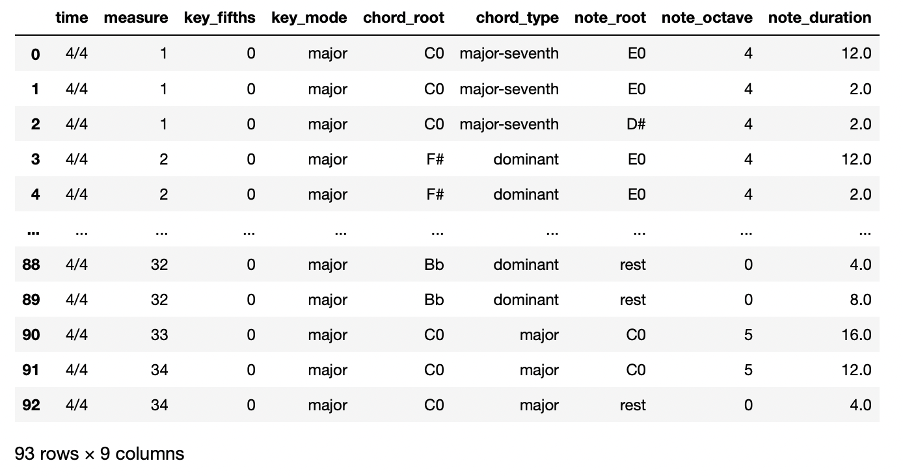
\includegraphics{Figures/CSV dataframe}
\decoRule
\caption{A song in DataFrame format after being read from CSV file}
\label{fig:CSV_DF}
\end{figure}

%-----------------------------------
%	SECTION 2
%-----------------------------------
\section{Preprocessing of dataset}

The dataset has to be preprocessed in order to make things simpler later on.

\begin{enumerate}
  \item All songs are transposed to C major key. The key of a song determines the notes and the set of chords present in the song. Transposing all songs to a common key will basically normalise the different features of melodies and chords in different songs. The number of chord types present in the dataset will be reduced, which will decrease the number of chord types during the training process. Each song can be shifted to a different key without loss of the song's subjective character by shifting all the pitches equally.
  \item The time signatures are all normalised. Different songs have different time signatures. To do so, each \emph{note\_duration} is multiplied by the reciprocal of the time signature \emph{time} to give a normalised note duration.
  \item Chord types are restricted to major and minor chords. All other chord types are converted to their most similar major or minor chords.
  \item Some measures in the dataset contain rest notes. These measures are removed from the dataset.
  \item Octave information is not required and is removed from the dataset.
  \item There are also some irregular notes present in the dataset such as 'B-2' and 'A2'. The numbers after the letters do not seem to represent octave information and the paper from which this dataset was obtained made no mention of them. Given that they represent a very small portion of the dataset, measures containing these irregular notes are also removed.
\end{enumerate}

%-----------------------------------
%	SUBSECTION 1
%-----------------------------------
Using \emph{Pandas} to remove the unwanted measures mentioned above and to normalise the note durations is a straightforward task. However, shifting all the songs to C major key is trickier. We would need to know the original key of the song, and then transposed the \emph{note\_root} and \emph{chord\_root} appropriately to C major key. The original keys of the songs are stated implicitly by their \emph{key\_fifths}; since we know all the songs are in major key and that each major key has a unique number of sharps/flats, the numberical value of \emph{key\_fifths} can be mapped to a specific major key as shown in Table \ref{tab:kf_map}. Note that there exist more values of \emph{key\_fifths} than shown, but preliminary analysis of the dataset shows that only integer values of \emph{key\_fifths} from -6 to 7 are present within it. We also create a mapping of the 12 notes to a numerical representation as shown in Table \ref{tab:note_map} to make the processing easier later.

Using Table \ref{tab:kf_map} \& \ref{tab:note_map}, we can list all the major keys present in the dataset and convert the pitches that exist within each major key into their numerical representations (which goes from 1 to 12 and then loops back to 1) as shown in Table \ref{tab:bigtable}. As expected, the differences between the pitches of the same key are consistent across all the major keys (e.g. the difference between Pitch 1 and Pitch 3 is always 4 for every major key), which shows that we can indeed tranpose a song to a different key by just shifting all the pitches equally. For each DataFrame row, we just have to convert \emph{key\_fifths} to the corresponding major key using \ref{tab:kf_map} to obtain the numerical representaion of Pitch 1 of that major key. We also convert \emph{note\_root} and \emph{chord\_root} to numbers using Table \ref{tab:note_map}. Next, the numerical representation of Pitch 1 is subtracted from those of \emph{note\_root} and \emph{chord\_root}, and the differences are added to Pitch 1 of the C major key (which is 1) to obtain the shifted pitches in notes and chords respectively. Note that the differences may be negative, which would lead to a shifted note/chord that is outside of the 1-12 range. This is easily rectified by using \emph{if} statements to check if the shifted note/chord is non-positive and to add 12 (since a zero would loop back to 12) to it if so.

The next step is to convert all the chord types to either major or minor chords using the mapping shown in Table \ref{tab:chords}. This mapping has been checked by the supervisors of this project and deemed to be reasonable. Do also note that Table \ref{tab:chords} does not contain an exhaustive list of all chords in existence, but only those that were found to be present within the dataset.

\subsection{Code}
As mentioned above, we first use \emph{Pandas} to clean up the data. A nested loop can then used to loop through each DataFrame row for each song. The steps outlined above can then be applied to each row. At the end of the nested loop, the dataset is now fully preprocessed.

%\begin{figure}
 %   \centering
  %  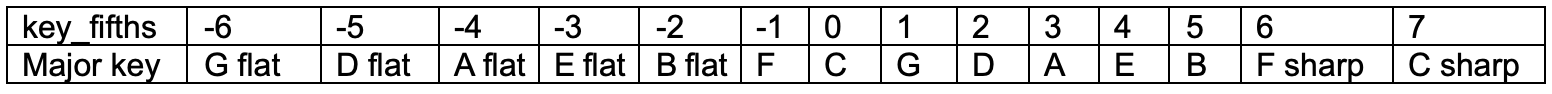
\includegraphics{Figures/key_fifths_mapping}
   % \decoRule
   % \caption{Mapping of \emph{key\_fifths} to major key}
   % \label{fig:kf_map}
    %\end{figure}

    \begin{table}
        \caption{Mapping of \emph{key\_fifths} to major key}
        \label{tab:kf_map}
        \centering
        \begin{tabular}{|c||c|c|c|c|c|c|c|c|c|c|c|c|c|c|}
        \hline
        \emph{key\_fifths} & -6 & -5 & -4 & -3 & -2 & -1 & 0 & 1 & 2 & 3 & 4 & 5 & 6 & 7 \\
        \hline
        Major key & Gb & Db & Ab & Eb & Bb & F & C & G & D & A & E & B & F\# & C\# \\
        \hline
        \end{tabular}
        \end{table}

\begin{table}
    \caption{Mapping of music notes to numerical representations}
    \label{tab:note_map}
    \centering
    \begin{tabular}{|c|c|c|c|c|c|}
    \hline
    C/B\# & C\#/Db & D & D\#/Eb & E/Fb & F/E\# \\
    \hline
    1 & 2 & 3 & 4 & 5 & 6 \\
    \hline
    \end{tabular}
    \begin{tabular}{|c|c|c|c|c|c|}
        \hline
    F\#/Gb & G & G\#/Ab & A & A\#/Bb & B/Cb\\
    \hline
    7 & 8 & 9 & 10 & 11 & 12\\
    \hline
    \end{tabular}
    \end{table}

    \begin{table}
        \caption{The component notes/pitches of each major key}
        \label{tab:bigtable}
        \centering
        \begin{tabular}{|c||c|c|c|c|c|c|c|}
        \hline
        Major key & Pitch 1 & Pitch 2 & Pitch 3 & Pitch 4 & Pitch 5 & Pitch 6 & Pitch 7 \\
        \hline
        \hline
        C\# & 2 & 4 & 6 & 7 & 9 & 11 & 1 \\
        \hline
        F\# & 7 & 9 & 11 & 12 & 2 & 4 & 6\\
        \hline
        B & 12 & 2 & 4 & 5 & 7 & 9 & 11\\
        \hline
        E & 5 & 7 & 9 & 10 & 12 & 2 & 4\\
        \hline
        A & 10 & 12 & 2 & 3 & 5 & 7 & 9\\
        \hline
        D & 3 & 5 & 7 & 8 & 10 & 12 & 2\\
        \hline
        G & 8 & 10 & 12 & 1 & 3 & 5 & 7\\
        \hline
        C & 1 & 3 & 5 & 6 & 8 & 10 & 12\\
        \hline
        F & 6 & 8 & 10 & 11 & 1 & 3 & 5\\
        \hline
        Bb & 11 & 1 & 3 & 4 & 6 & 8 & 10\\
        \hline
        Eb & 4 & 6 & 8 & 9 & 11 & 1 & 3\\
        \hline
        Ab & 9 & 11 & 1 & 2 & 4 & 6 & 8\\
        \hline
        Db & 2 & 4 & 6 & 7 & 9 & 11 & 1\\
        \hline
        Gb & 7 & 9 & 11 & 12 & 2 & 4 & 6\\
        \hline
        \end{tabular}
        \end{table}

        \begin{table}
            \caption{Mapping of chords present within the dataset to major/minor chord.}
            \label{tab:chords}
            \centering
            \begin{tabular}{l l}
            \toprule
            Major & Minor \\
            \midrule
            Dominant-ninth & Minor-seventh\\
            Major-sixth & Minor-sixth\\
            Major-seventh & Diminished\\
            Dominant & Half-diminished\\
            Suspended-fourth & Minor-ninth\\
            Augmented-seventh & Diminished-seventh\\
            Major-ninth & Minor-eleventh\\
            Dominant-seventh & Minor-major\\
            Augmented & Major-minor\\
            Dominant-thirteenth & Minor-thirteenth\\
            Power & Minor seven flat five\\
            Suspended-second &  \\
            Dominant-eleventh &  \\
            Pedal &  \\
            Major 6/9 &  \\
            Augmented-ninth &  \\
            Sixth &  \\

            \bottomrule\\
            \end{tabular}
            \end{table}
            

        \begin{figure}
            \centering
            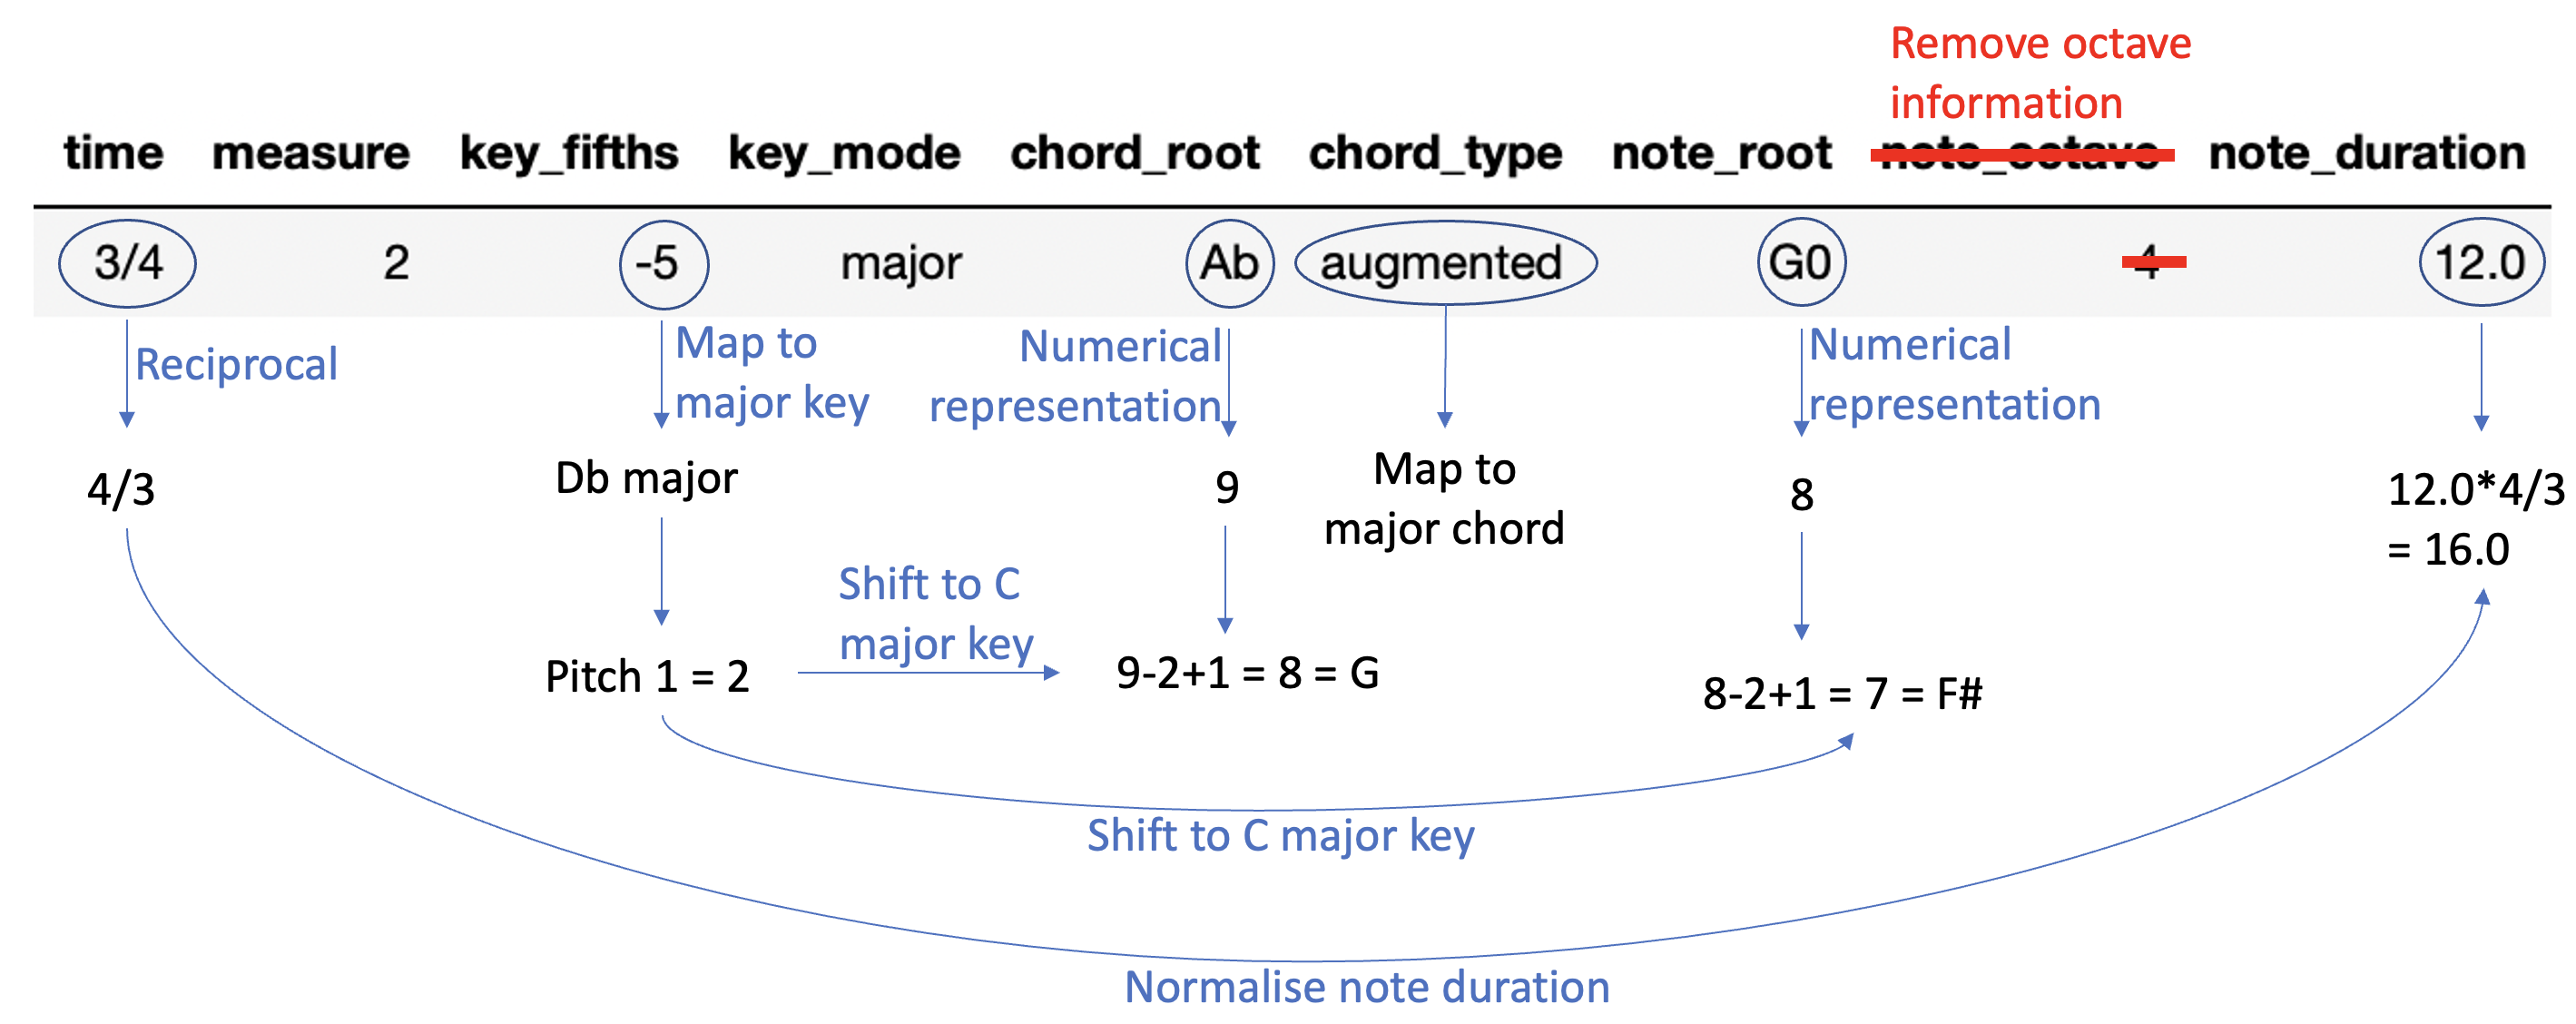
\includegraphics[scale=0.3]{Figures/Algorithm pictorial2}
            \decoRule
            \caption{Pictorial representation of the preprocessing of the dataset.
            }
            \label{fig:Alg1}
            \end{figure}
            
%-----------------------------------
%	SUBSECTION 2
%-----------------------------------

%\subsection{Subsection 2}
%Morbi rutrum odio eget arcu adipiscing sodales. Aenean et purus a est pulvinar pellentesque. Cras in elit neque, quis varius elit. Phasellus fringilla, nibh eu tempus venenatis, dolor elit posuere quam, quis adipiscing urna leo nec orci. Sed nec nulla auctor odio aliquet consequat. Ut nec nulla in ante ullamcorper aliquam at sed dolor. Phasellus fermentum magna in augue gravida cursus. Cras sed pretium lorem. Pellentesque eget ornare odio. Proin accumsan, massa viverra cursus pharetra, ipsum nisi lobortis velit, a malesuada dolor lorem eu neque.

%----------------------------------------------------------------------------------------
%	SECTION 3
%----------------------------------------------------------------------------------------

\section{Model input format}
Now that the dataset has been preprocessed, it can now be converted into a format that is appropriate for input to the machine learning model.

\subsection{LSTM format}
The LSTM data input format is a matrix with 37 columns, with each row containing informaion about a single measure. The first 12 columns represent the 12 note (C,C\#, etc.), the next 24 columns represent the 12 major chords and the 12 minor chords, and the last column correspond to the absence of a chord. If a particular note exists within a particular measure, the element that corresponds to that particular measure (row) and particular note (column) will be the normalised duration of that note. Similarly, the element that corresponds to the chord of a particular measure will be a '1'. Notes and chords that are not present within that measure will be marked with a '0'. If no chords are present within a measure, the last column will be marked as a '1'. A pictorial representation of the transformation is shown in Figure \ref{fig:LSTMData}.

\subsubsection{Code}
We again use a nested loop to loop through each DataFrame row for each song. Two 1 by 37 arrays \emph{LSTM\_data} and \emph{new\_row} are initialised. As we loop through each row, we keep track of the meaasure. As long as the measure does not change, \emph{new\_row} is progressively updated with the normalised note durations of the present notes in this manner: $\emph{new\_row}[0,\emph{note}-1] = \emph{new\_row}[0,\emph{note}-1] + \emph{normalised\_note\_duration}$, where \emph{note} is the numerical representation of the note present in each DataFrame row and \emph{normalised\_note\_duration} is the normalised note duration of that note. This works because the mapping between the notes and their numerial representation starts at 1 and ends at 12 (as can be seem in Table \ref{tab:note_map}) and indexing starts at zero in Python. Hence, the (\emph{note}-1)\textsuperscript{th} column of the LSTM format (and thereby \emph{new\_row}) will correspond to \emph{note}.

Once the measure changes, the now complete \emph{new\_row} for the previous measure is concatenated with \emph{LSTM\_row} along the row axis, i.e. \emph{new\_row} is added to the bottom of \emph{LSTM\_row}. The elements of \emph{new\_row} are reset to zero before \emph{new\_row} is updated with the note and chord information of the current measure. The note information can be updated as explained earlier. For the chord information, we can use \emph{if} statements to set $\emph{new\_row}[0, \emph{chord}+11] = 1$ if \emph{chordtype} = 'major', or to set $\emph{new\_row}[0, \emph{chord}+23] = 1$ if \emph{chordtype} = 'minor', or to set $\emph{new\_row}[0, -1] = 1$ otherwise (no chord present), where \emph{chord} is the numerical representation of \emph{chord\_root} (mapped using Table \ref{tab:note_map}). Since we know that there is only one chord type per measure, we only have to update the chord information for \emph{new\_row} once, at the start of a new measure. The start of the first measure can be taken to be a special case of a measure change (in this case, transition from a measure initialised as 'unknown' to the first measure of the DataFrame).

%$\emph{new\_row}[0,\emph{note}-1] = \emph{new\_row}[0,\emph{note}-1] + \emph{normalised\_note\_duration}$
\begin{figure}
    \centering
    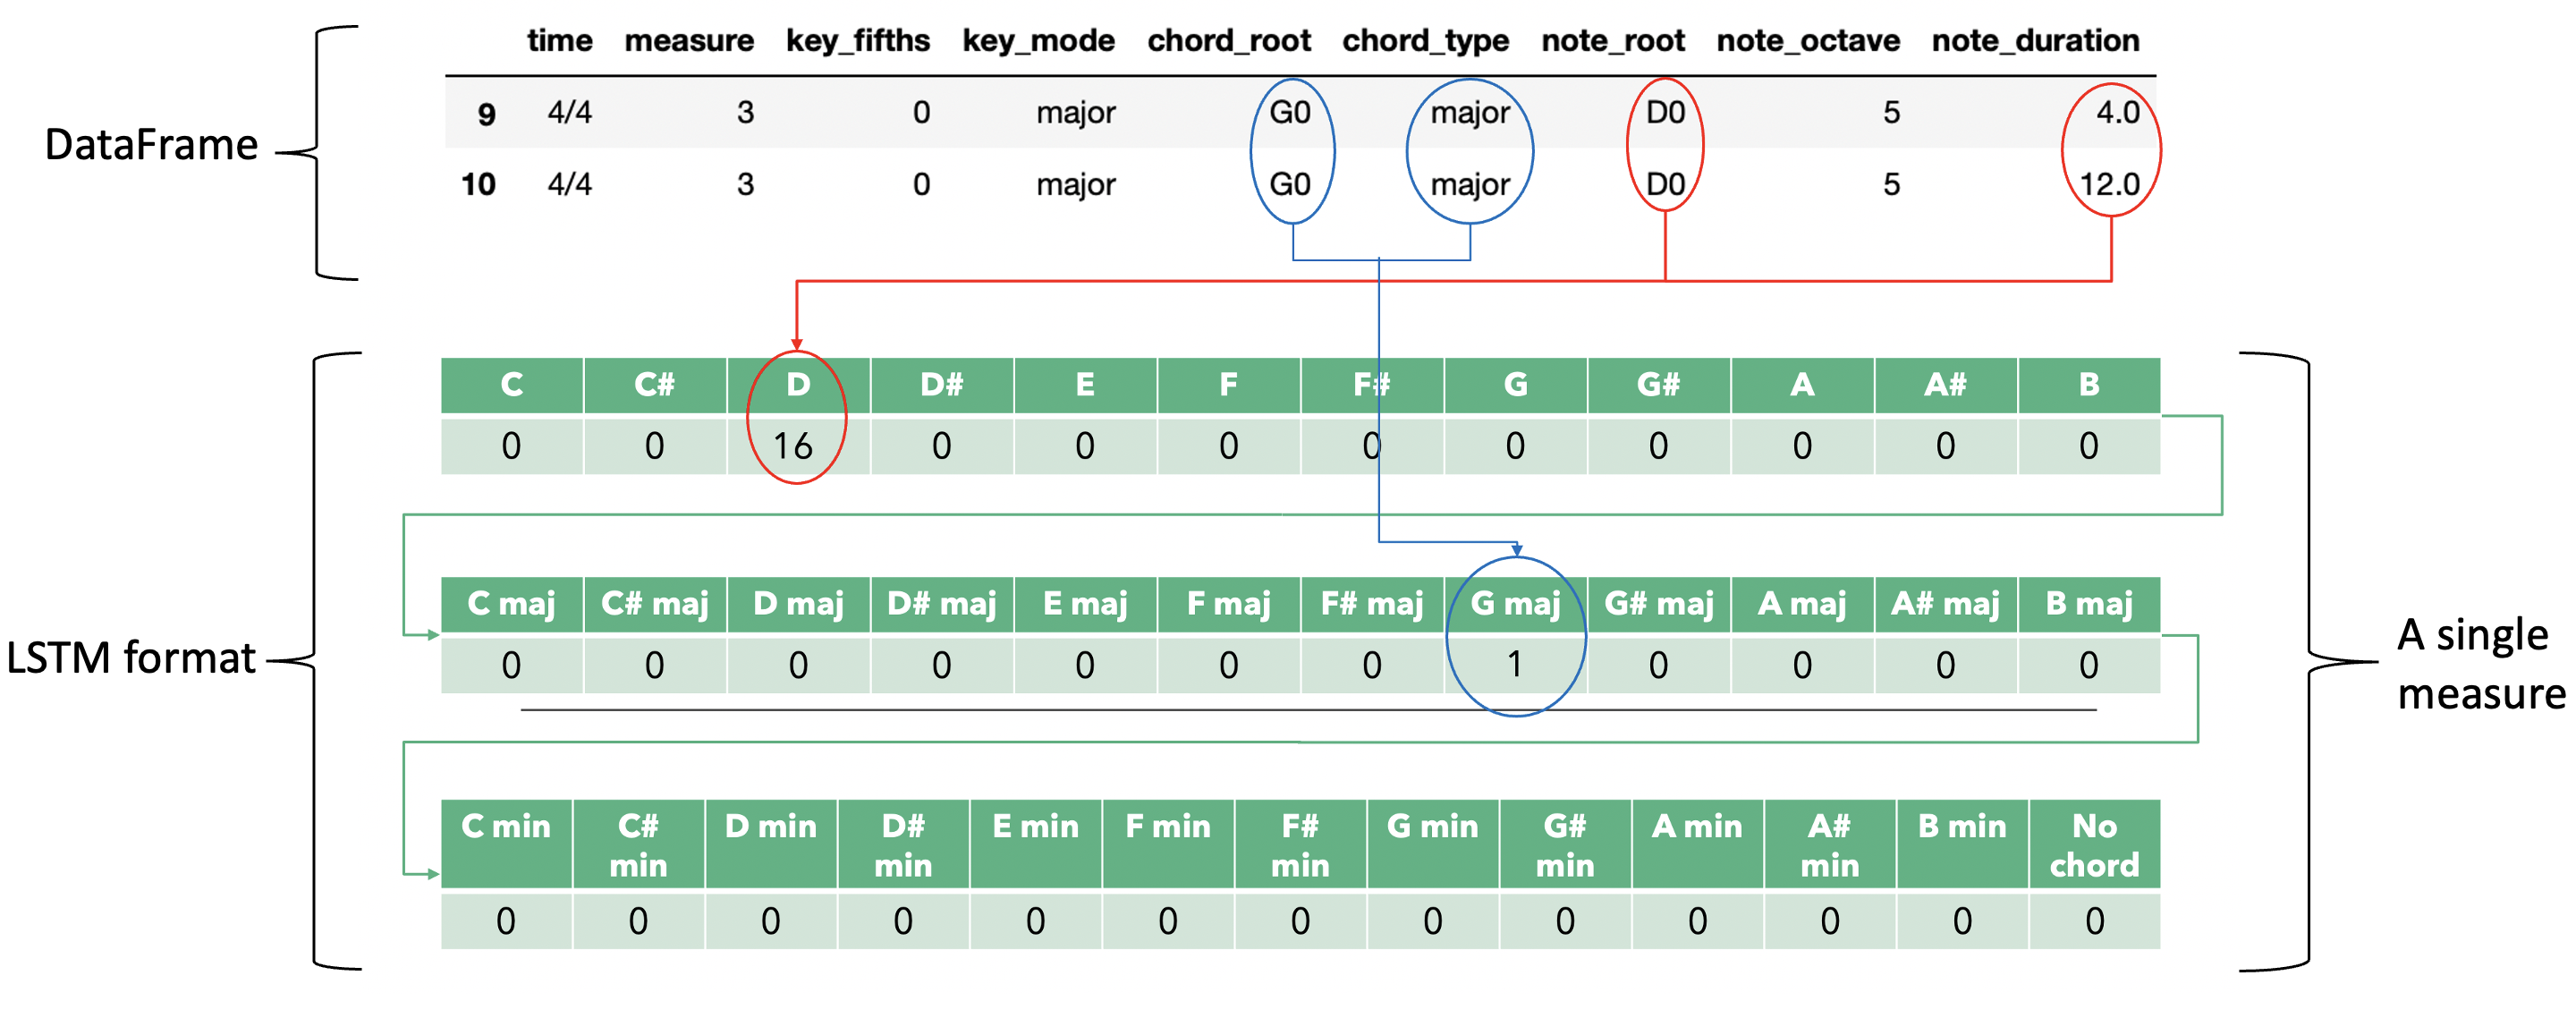
\includegraphics[scale=0.3]{Figures/LSTM pictorial 4}
    \decoRule
    \caption{Transforming DataFrame to LSTM data input format.}
    \label{fig:LSTMData}
\end{figure}
    


\subsection{Transformer format}
The transformer requires two data inputs: a single sequence of notes for each song, and a separate sequence of chords for eaach song. Both sequences are constructed by going down the Dataframe rows, and adding the notes/chords of each row to the respective sequences based on the \emph{note\_duration} value, e.g. a sequence of 4 'C\#'s for a 'C\#' with a \emph{note\_duration} of 4.0, and a sequence of 16 'Bmaj' for a 'B major' of \emph{note\_duration} of 16.0. Another example is presented in Figure \ref{fig:TransformerData}. Of course, this means that only integer values of \emph{note\_duration} are accepted and measures with non-integer values have to be removed beforehand.

It is obvious that the sequences will be very long given that just the three rows in Figure \ref{fig:TransformerData} resulted in 16 elements for each sequence. As shown in Chapter 4, the time complexity of the Transformer is ${n}^2$. Hence, it is crucial to reduce the sequence length to shorten the training time. This can be achieved by dividing all \emph{note\_duration} by their largest common factor for all measures within a single song. This may not reduce the length of the sequences for all songs (songs with \emph{note\_duration of 1.0} will have a trivial largest common factor of 1.0), but it will still reduce the sequence length for some songs, as shown in Figure \ref{fig:Transformer LCF}, which will decrease the training time significantly.


\begin{figure}
    \centering
    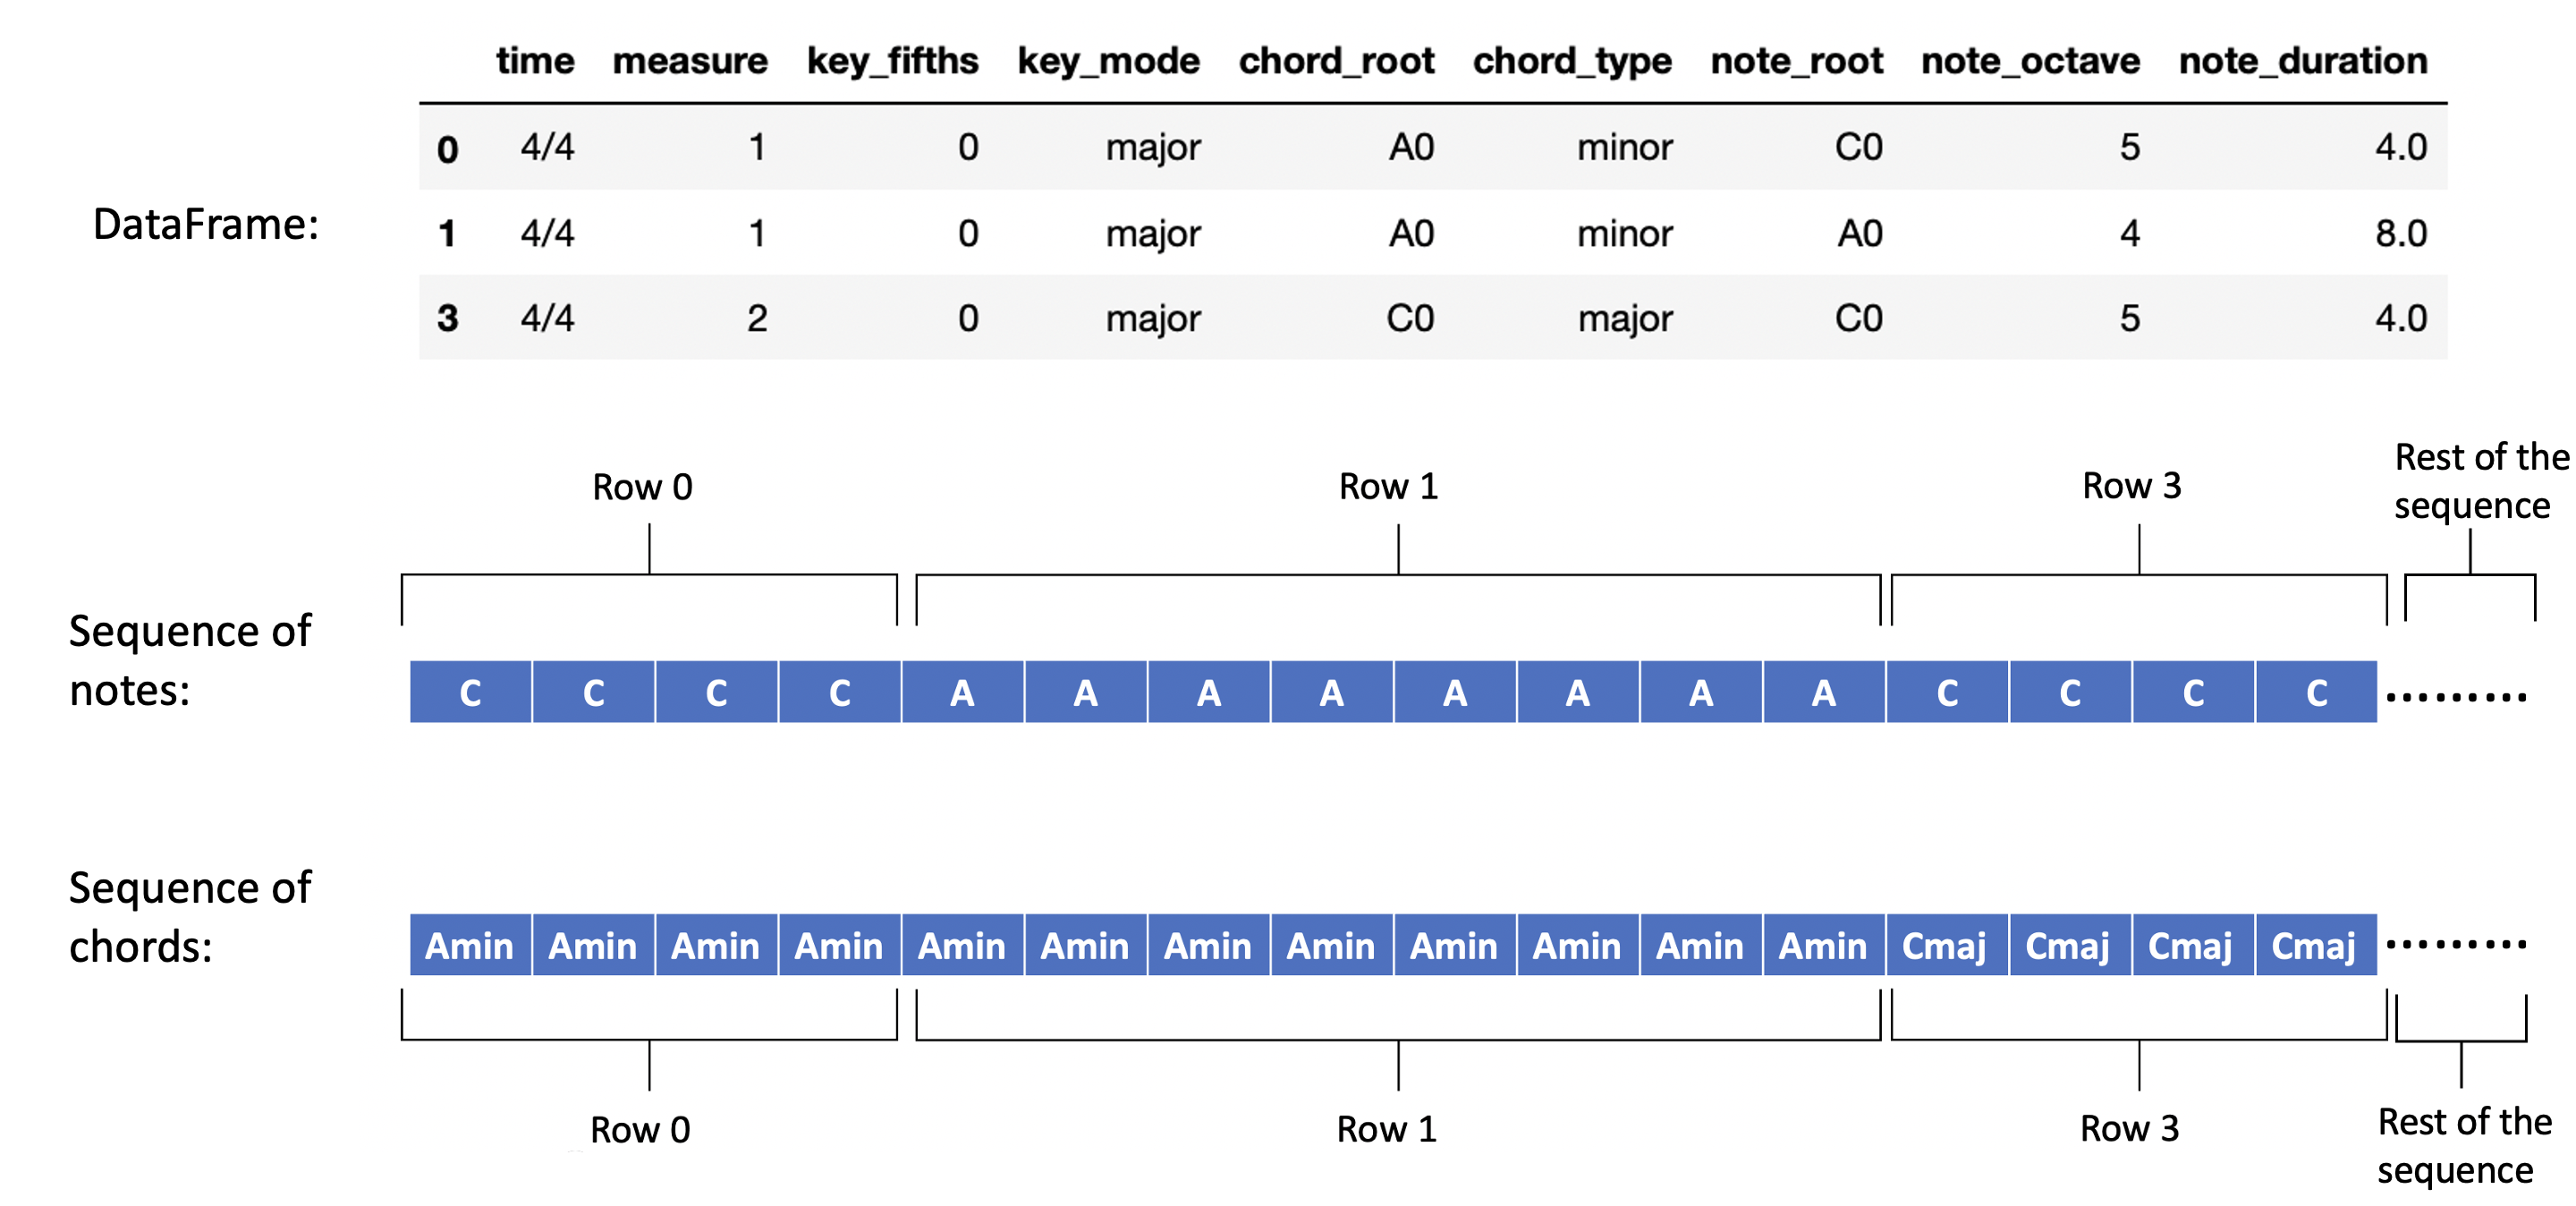
\includegraphics[scale=0.3]{Figures/Transformer 2}
    \decoRule
    \caption{Converting DataFrame to Transformer data input format.}
    \label{fig:TransformerData}
    \end{figure}

\begin{figure}
    \centering
    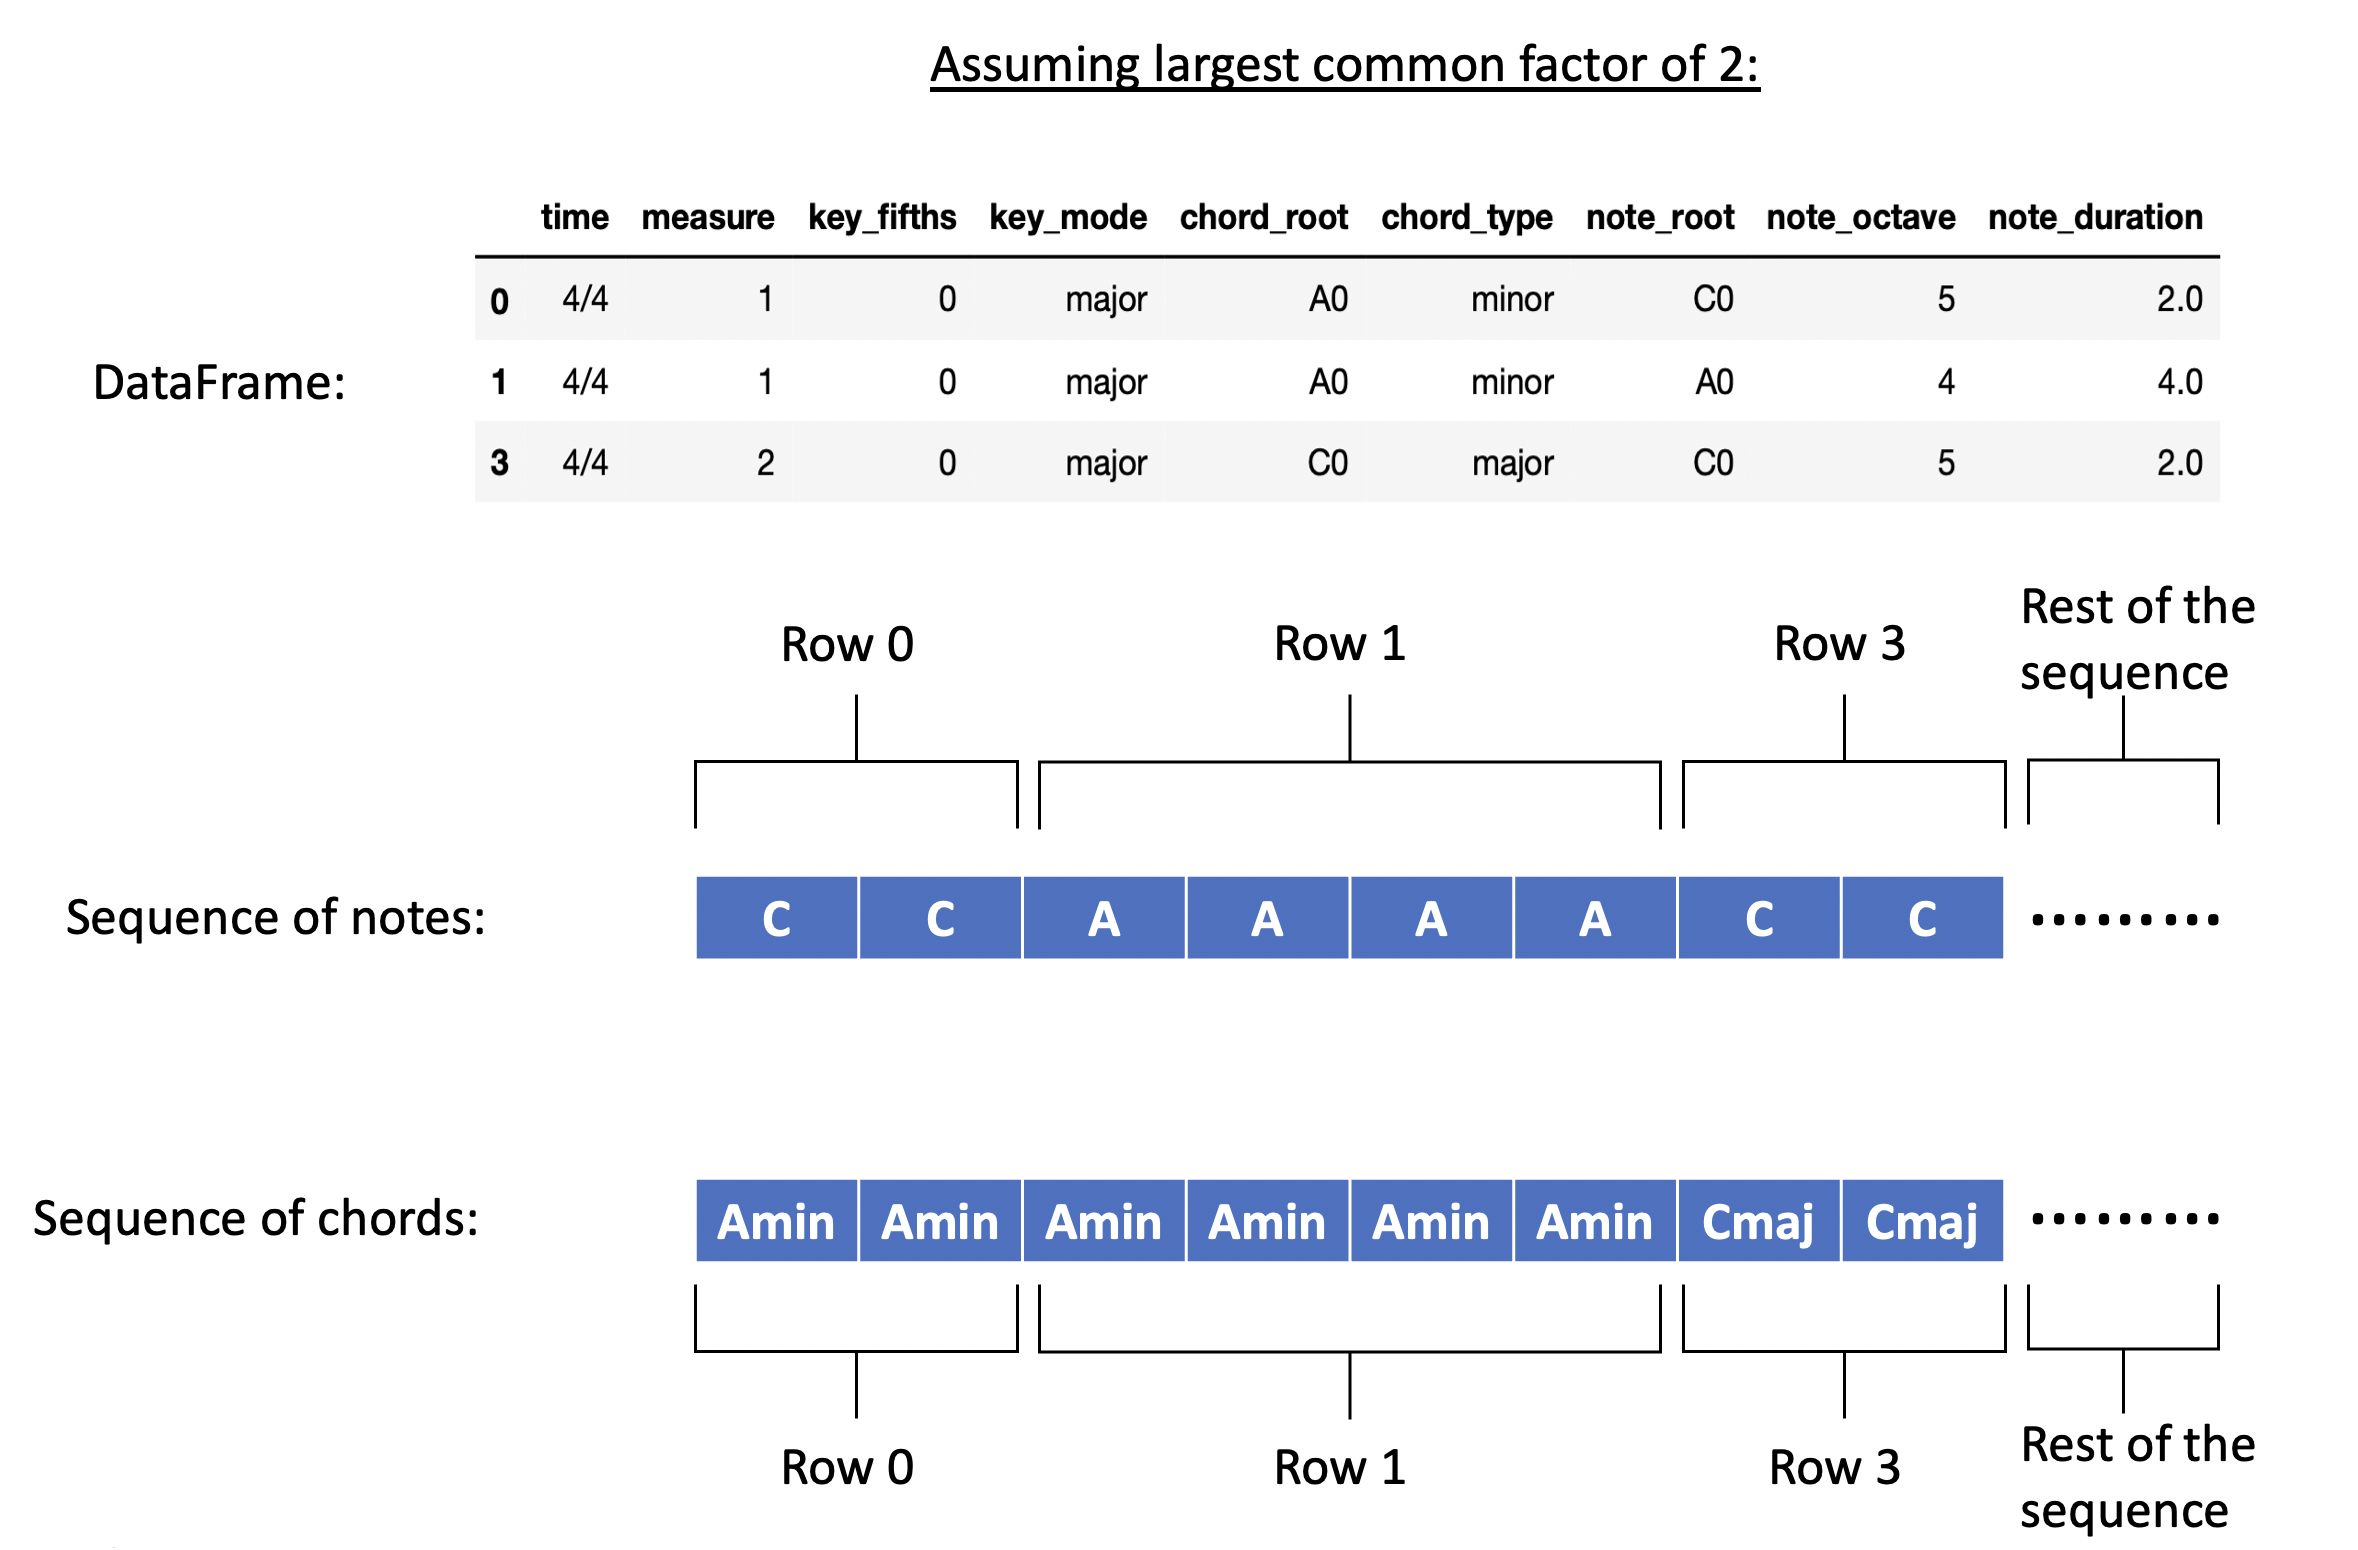
\includegraphics[scale=0.3]{Figures/Transformer LCF}
    \decoRule
    \caption{Converting DataFrame (normalised by the largest common factor) to Transformer data input format.}
    \label{fig:Transformer LCF}
    \end{figure}

\subsubsection{Code}
The same nested loop as before is used again for this. Four empty lists \emph{note\_duration\_li}, \emph{note\_li}, \emph{chord\_li}, \emph{chordtype\_li} are initialised. As we loop through the DataFrame rows of a single song, we append the information from each row to the respective lists. At the end of this inner loop, the largest common factor of \emph{note\_duration\_li} can be found using the \emph{math.gcd} function. Since \emph{math.gcd} only accepts two arguments, we initialise \emph{lcf} as the index 0 element of \emph{note\_duration\_li}, and loop from the index 1 element to the last element of \emph{note\_duration\_li}. Within this loop, \emph{math.gcd} takes in \emph{lcf} and \emph{note\_duration\_li}[\emph{j}] as its two arguments, where \emph{j} is the currect loop index. In essence, we are just finding the largest common factor of the first two elements of \emph{note\_duration\_li}, and finding the largest common factor of the previous largest common factor and the third element, and so on. This will give us the largest common factor of all the values stored in \emph{note\_duration\_li}, which are all then divided by this largest common factor to give \emph{normalised\_note\_duration}.

We can now start to construct the sequences of notes and chords. Two empty arrays \emph{row\_note} and \emph{row\_chord} are initialised, and we loop through \emph{normalised\_note\_duration} with loop index \emph{k}. For the \emph{k}\textsuperscript{th} element of \emph{normalised\_note\_duration}, a 1 by \emph{normalised\_note\_duration}[\emph{k}] array filled with '1's is initialised and multiplied by \emph{note\_li}[\emph{k}]. The result is concatenated with \emph{row\_note} along the column axis. For the chord sequence, a 1 by \emph{normalised\_note\_duration}[\emph{k}] array filled with '1's is also initialised. This array is multiplied by \emph{chord\_li}[\emph{k}] if chordtype\_li[\emph{k}] is 'major', by $(\emph{chord\_li}[\emph{k}] + 12)$ if it is 'minor', and zero if there are no chords. The resulting array is then concatenated with \emph{row\_chord} along the column axis.

After looping through all the DataFrame rows of a song, \emph{row\_note} and \emph{row\_chord} are the now complete sequences of notes and chords respectively for that song. These will be the input to the Transformer model.